\documentclass{emulateapj}
%\documentclass[12pt,preprint]{aastex}

\usepackage{graphicx}
\usepackage{float}
\usepackage{amsmath}
\usepackage{epsfig,floatflt}
\usepackage{hyperref}
\usepackage[toc, page]{appendix}
\usepackage{verbatim, amsmath, amsfonts, amssymb, amsthm}
\usepackage[utf8]{inputenc}
\usepackage{textcomp}
\usepackage{float}
\usepackage{xcolor}
\usepackage{color}
\usepackage{listings}
\usepackage{fancyhdr}
\usepackage[T1]{fontenc}
\usepackage{url}
\usepackage[export]{adjustbox}
\usepackage{calc}
\usepackage{caption}

\usepackage{accents}
\newcommand{\dbtilde}[1]{\accentset{\approx}{#1}}
\newcommand{\vardbtilde}[1]{\tilde{\raisebox{0pt}[0.85\height]{$\tilde{#1}$}}}

\usepackage{lipsum}
\usepackage[para]{footmisc}


\definecolor{mygreen}{rgb}{0,0.6,0}
\definecolor{mygray}{rgb}{0.5,0.5,0.5}
\definecolor{mymauve}{rgb}{0.58,0,0.82}

\lstset{ %
	backgroundcolor=\color{white}\ttfamily\tiny,   % choose the background color; you must add \usepackage{color} or \usepackage{xcolor}; should come as last argument
	basicstyle=\tiny,        % the size of the fonts that are used for the code \footnotesize,
	breakatwhitespace=false,         % sets if automatic breaks should only happen at whitespace
	columns=fullflexible,    %no spaces between columns
	keepspaces=true,
	breaklines=true,                 % sets automatic line breaking
	breakatwhitespace=true,
	captionpos=b,                    % sets the caption-position to bottom
	commentstyle=\color{mygreen},    % comment style
	deletekeywords={...},            % if you want to delete keywords from the given language
	escapeinside={\%*}{*)},          % if you want to add LaTeX within your code
	extendedchars=true,              % lets you use non-ASCII characters; for 8-bits encodings only, does not work with UTF-8
	frame=single,	                   % adds a frame around the code
	keepspaces=true,                 % keeps spaces in text, useful for keeping indentation of code (possibly needs columns=flexible)
	keywordstyle=\color{blue},       % keyword style
	language=Python,                 % the language of the code
	morekeywords={*,...},           % if you want to add more keywords to the set
	%numbers=left,                    % where to put the line-numbers; possible values are (none, left, right)
	%numbersep=5pt,                   % how far the line-numbers are from the code
	%numberstyle=\tiny\color{mygray}, % the style that is used for the line-numbers
	rulecolor=\color{black},         % if not set, the frame-color may be changed on line-breaks within not-black text (e.g. comments (green here))
	showspaces=false,                % show spaces everywhere adding particular underscores; it overrides 'showstringspaces'
	showstringspaces=false,          % underline spaces within strings only
	showtabs=false,                  % show tabs within strings adding particular underscores
	stepnumber=1,                    % the step between two line-numbers. If it's 1, each line will be numbered
	stringstyle=\color{mymauve},     % string literal style
	tabsize=1,	                   % sets default tabsize to 2 spaces
	%title=\lstname                   % show the filename of files included with \lstinputlisting; also try caption instead of title
}

\begin{document}

\title{Numerical integration - An empirical study of Gaussian quadrature and Monte Carlo}

\author{Bruce Chappell and Markus Bjørklund}

\email{markus.bjorklund@astro.uio.no}

\altaffiltext{1}{Institute of Theoretical Astrophysics, University of
  Oslo, P.O.\ Box 1029 Blindern, N-0315 Oslo, Norway}

\begin{abstract}

In this paper, we apply the Gaussian quadrature and Monte Carlo integration methods for solving the six-dimensional integral arising from the expectation value for the correlation energy between two electrons in a helium atom. The results show that neither the Brute force Gaussian nor the brute force Monte Carlo reaches the accuracy of three leading decimal points, up to $N=60$ and $N=10^8$ respectively. The improved Gaussian reaches the desired accuracy already at N=30 grid points, with a run time of 67.605 seconds, while the improved Monte Carlo reaches three-decimal point accuracy for $N=10^{6}$ with a run time of 0.504 seconds. This shows that for multi-dimensional integrals of this order, the improved Monte Carlo is clearly the preferred method of integration.

\end{abstract}
\keywords{Numerical integration --- Guassian quadrature --- Monte Carlo methods}

\section{Introduction}
\label{sec:introduction}

In many scientific applications, we encounter the case of multi-dimensional integrals. These are almost always impossible to solve analytically, so we need to employ numerical methods. Traditional integration methods, like Newton-Cotes, often require a lot of mesh points in order to achieve a desired accuracy, thereby drastically increasing the demand for computational power. In the case of multi-dimensional integrals, this demand would be even higher, as we would scale as $N^n$ FLOPS, where N is the number of mesh points and n is the dimension of the integral. Therefore, there is a lot to be gained by finding methods in which we can decrease the amount of FLOPS, while retaining the accuracy. In this paper, we will look at two such methods here, namely Gaussian quadrature and Monte Carlo integration.

The problem in question is that of determining the ground state correlation energy between two electrons in a helium atom. This problem presents a six-dimensional integral, with an analytical solution. The fact that an analytical solution exists will prove as an important benchmark for our algorithms, and thereby sets up a perfect environment for testing the efficiency of different algorithms.

The paper consists of 5 main sections following this one. In the theory section, we provide the fundamental theory for setting up the problem, as well as the theory behind the algorithms used to solve the integral. In the methods section, we present details on the implementation of the algorithms, and the choice of parameters, as well as unit testing. In the results section, we provide the main results, focusing on numerical result, error and run time. We discuss the results in the discussion section, and provide closing thoughts in the conclusions section.
\section{Theory}
\label{sec:method}
Our first assumption is that each electron behaves according to the single-particle wave function for an electron in the hydrogen atom, albeit not normalized, given as

\[
   \psi_{1s}({\bf r}_i)  =   e^{-\alpha r_i},
\]
where
\[
   {\bf r}_i =  x_i {\bf e}_x + y_i {\bf e}_y +z_i {\bf e}_z ,
\]
and
\[
r_i = \sqrt{x_i^2+y_i^2+z_i^2}.
\]

Here, $\alpha$ is a parameter. We fix $\alpha$ as a parameter denoting the charge, and in the case of the helium atom, we have $\alpha = 2$. Our ansatz for the combined wave function is that it is given by the product of the individual wave functions
\[
   \Psi({\bf r}_1,{\bf r}_2)  =   e^{-2 (r_1+r_2)}.
\]
Then, the correlation energy, and the integral we wish to solve, is defined as
\begin{equation}\label{eq:correlationenergy}
   \langle \frac{1}{|{\bf r}_1-{\bf r}_2|} \rangle =
   \int_{-\infty}^{\infty} d{\bf r}_1d{\bf r}_2  e^{-4 (r_1+r_2)}\frac{1}{|{\bf r}_1-{\bf r}_2|}.
\end{equation}
This is a six dimensional integral, and has the closed form analytical solution
\[
\langle \frac{1}{|{\bf r}_1-{\bf r}_2|} \rangle = \frac{5\pi^2}{16^2}
\]

\subsection{Gaussian quadrature}
Our first approach is to integrate using Gaussian quadrature. Gaussian quadrature, unlike Newton-Cotes methods, generally have non-evenly spaced integration points $\{x_0 , x_1 , \dots , x_{N-1}\}$, given by the zeros of an orthogonal polynomial. The integral is then approximated by
\begin{equation}
	I = \int_a^b f(x) dx \approx \sum^N_{i = 1} \omega_i f(x_i),
	\label{eq:quadrature}
\end{equation}
where $\omega_i$ are the integration weights.

\subsubsection{Integration points and weights}
There are N integration points and N integration weights. We must therefore approximate the function with a polynomial of degree $2N-1$, $f(x) \approx P_{2N-1}$ to find them. Gaussian quadrature is exact when integrating a polynomial (up to the same degree), and we get

\begin{align}
	I \approx \int P_{2N-1}(x)dx = \sum^{N-1}_{i=0}P_{2N-1}(x_i) \omega_i.
\end{align}

The idea is to expand this polynomial in terms of some (often known) other polynomial of degree N through polynomial division. The choice of polynomial depends on the integration limits, which sets the scope of the orthogonal polynomial. We use the Legendre polynomial $L_N(x)$ here, which is orthogonal for $x\in [-1,1]$, but the argument is valid for all orthogonal polynomials.
\begin{equation}
	P_{2N-1} = L_N(x)P_{N-1}(x) + Q_{N-1}(x),
\end{equation}
where $Q_{N-1}(x)$ is the remainder from the polynomial division. It can be shown, see \cite{Lecture1}, that the weights are given by

\begin{equation}
    w_i = 2\left(\hat{L}^{-1}\right)_{0,i},
\end{equation}
where $\hat{L}$ is the matrix
\begin{equation*}
   \hat{L}=\left(\begin{array} {cccc} L_0(x_0)  & L_1(x_0) &\dots &L_{N-1}(x_0)\\
                                   L_0(x_1)  & L_1(x_1) &\dots &L_{N-1}(x_1)\\
                                   \dots  & \dots &\dots &\dots\\
L_0(x_{N-1})  & L_1(x_{N-1}) &\dots &L_{N-1}(x_{N-1})
\end{array}\right),
\end{equation*}
and the integration points $x_i$ are the zeros of the polynomial $L_N$. For the general case of limits
\begin{equation}
    \int_a^b f(t) dt,
\end{equation}
one can always perform the mapping $t = \frac{b-a}{2}x + \frac{b+a}{2}$ to obtain

\begin{equation*}
  \int_a^bf(t)dt=\frac{b-a}{2}\int_{-1}^1f\left(\frac{(b-a)x}{2}+\frac{b+a}{2}\right)dx.
\end{equation*}

\subsection{Transformation to spherical coordinates}
Our original integral is not well suited for the use of Legendre polynomials. It would therefore be reasonable to perform a transformation to spherical coordinates, and employ the Laguerre polynomials, which are orthogonal on the interval $[0,\infty)$. The Laguerre polynomials are well suited to solve integrals on the form
\begin{equation}
    \int_0^\infty f(x) e^{-x} dx.
\end{equation}

In spherical coordinates, the new differentials become
\begin{align*}
    d\vec{r}_1d\vec{r}_2 &= r_1^2r_2^2 dr_1dr_2 d\cos(\theta_1)d\cos(\theta_2) d\phi_1d\phi_2 \\
    &= r_1^2r_2^2 dr_1dr_2\sin(\theta_1)\sin(\theta_2)d\theta_1d\theta_2d\phi_1d\phi_2
\end{align*}
and the distance between the electrons is given by
\begin{equation*}
|\vec{r}_1 - \vec{r}_2| = \sqrt{r_1^2 + r_2^2 - 2r_1r_2cos(\beta)},
\end{equation*}
where
\begin{equation*}
cos(\beta) = cos(\theta_1)\cos(\theta_2) + \sin(\theta_1)\sin(\theta_2)\cos(\phi_1 - \phi_2).
\end{equation*}

We introduce the substitution $u = 2\alpha r$, such that $r^2 = \frac{u^2}{4\alpha^2}$ and $dr = \frac{du}{2\alpha}$. Inserting all this, we get the integral
\begin{equation}
    I = \frac{1}{32\alpha^5}\int_0^\pi \int_0^\pi \int_0^{2\pi} \int_0^{2\pi} \int_0^{\infty} \int_0^{\infty} f du_1 du_2 d\phi_1 d\phi_2 d\theta_1 d\theta_2,
\end{equation}
where
\begin{equation}
    f = \frac{u_1^2 u_2^2 sin\left(\theta_1\right) sin\left(\theta_2\right) e^{-\left(u_1+u_2\right)}}{\sqrt{u_1^2 + u_2^2 - 2u_1u_2cos\left(\beta\right)}}.
\end{equation}
with new limits $\theta_{1,2} \in [0,\pi]$, $\phi_{1,2} \in [0,2\pi]$ and $r_{1,2} \in [0,\infty)$ as per usual in spherical coordinates. Thus, it is appropriate to use Laguerre polynomials for the radial part, and Legendre polynomials with a mapping to $[-1,1]$ for the angular parts.

\subsection{Monte Carlo integration}
The idea behind Monte Carlo integration is that we can approximate an integral

\begin{equation} \label{eq:MC}
    \int_a^b f\left(x\right) P\left(x\right) \approx \frac{1}{N}\sum_{i=0}^{N-1} f\left(x_i\right),
\end{equation}
where $x_i$ is drawn from the probability distribution $P\left(x\right)$, and N denotes the number of samples. For the case where there is no known distribution inside the integral, one must choose one, I.E.

\begin{equation}
    \int_a^b f\left(x\right) = \int_a^b \frac{f\left(x\right)}{P\left(x\right)}P\left(x\right) dx \equiv \int_a^b g\left(x\right) P\left(x\right) dx.
\end{equation}
Assuming a uniform distribution,
\begin{equation}
    P_\text{uniform}(x) = \frac{1}{b-a}\theta\left(x-a\right)\theta\left(b-x\right),
\end{equation}
where $\theta$ denotes the Heaviside step function, we get

\begin{equation}
    \int_a^b f(x) dx = \left(b-a\right) \int_a^b f(x) P_\text{uniform}(x) dx.
\end{equation}
In the case of the correlation energy, we have $(a,b) = (-\infty,\infty)$, a 6-dimensional integral and our original integrand as given in equation \ref{eq:correlationenergy}. Thus we need to again approximate the limits as $(-\lambda,\lambda)$, and we get

\begin{align*}
    I &= \left(2\lambda\right)^6 \int_{-\lambda}^{\lambda} d{\bf r}_1d{\bf r}_2  e^{-4 (r_1+r_2)}\frac{1}{|{\bf r}_1-{\bf r}_2|} P_\text{uniform}({\bf r}_1, {\bf r}_2) \\
    &= \left(2\lambda\right)^6 \int_{-\lambda}^{\lambda} d{\bf r}_1d{\bf r}_2 f({\bf r}_1, {\bf r}_2) P_\text{uniform}({\bf r}_1, {\bf r}_2)
\end{align*}
Thus, we can apply Monte Carlo integration by the relation in equation \ref{eq:MC}, and obtain that
\begin{equation}
    I \approx \frac{\left(2\lambda\right)^6}{N}\sum_{i=0}^{N-1} f({\bf r}_{1,i}, {\bf r}_{2,i}),
\end{equation}
where $\bf r_i$ is drawn from the uniform distribution (I.E. each variable $x_1$, $x_2$, $y_1$, ...).

\subsection{Importance sampling}
As in the case of the Legendre polynomial for the radial part of the integral, we again face a situation where our sample interval, represented by the uniform distribution, does not fit our integrand very well. Therefore, it would be logical to apply "Importance sampling". Importance sampling is the process of drawing from a distribution that follows the shape of the integrand, or in other words "sampling the important values".

We recognize that our integrand contains an exponential term. Probability is conserved under transformation of variables, so by calling

\begin{equation}
    P(y) = e^{-y}
\end{equation}
our probability density function, and mapping
\begin{equation}
    y(u) = -ln\left(1-u\right),
\end{equation}
we get our new integral variable $y\in [0,\infty)$, and can perform Monte Carlo integration with drawing from the exponential distribution instead. This is done for the radial part which has limits $[0,\infty)$, while the angular part still is drawn from the uniform distribution.

\section{Methods}
\label{sec:methods}
In this section we will describe the methods we utilized to acquire our results.
\subsection{Code}
The code used to acquire the results in this report comes from the C++ program \texttt{num\_int.cpp}. This file executes various numerical integration methods, runs unit tests, and prints results to text files. A similar program, \texttt{parallel.cpp}, performs Monte-Carlo integration on parallel cores. There is also a python file \texttt{plot.py} that is used to put the data into easy to handle Pandas dataframes and plot the results.

\subsection{Algorithm}
The C++ program \texttt{num\_int.cpp} solves one integration problem using four different methods: Gauss-Legendre Quadrature, a mix of Gauss-Legendre and Gauss-Laguerre Quadrature which we will call Improved Gaussian Quadrature, Monte-Carlo integration using the uniform distribution, and Monte-Carlo integration using importance sampling.
\subsubsection{Quadrature}
For the less elegant Gaussian Quadrature methods, we use functions \texttt{gauss\_legendre} and \texttt{gauss\_laguerre} found in \cite{codeex} to calculate the integration points and weights for both Gaussian-Legendre and Improved Gaussian Quadrature. The brute force Gaussian-Legendre Quadrature is done using the following pseudo code.
\begin{lstlisting}[language=c++]
double brute_force(int N, double a, double b){
    double *x = new double [N];
    double *w = new double [N];
    gauss_legendre(a, b, x, w, N);
    for (int i = 0; i < N; i++){
        for (int j = 0; j < N; j++){
          for (int k = 0; k < N; k++){
            for (int l = 0; l < N; l++){
              for (int m = 0; m < N; m++){
                for (int n = 0; n < N; n++){
                  integral += w[i]*w[j]*w[k]*w[l]*w[m]*w[n]
                            * remainder(x[i],x[j],x[k],x[l],x[m],x[n]);
    }}}}}}}
\end{lstlisting}
Here we have integrated over all six spatial Cartesian variables on the interval $[a,b]$ with $N$ integration points. $remainder()$ is the remaining function after dividing out the weight function from the function of interest, $Q_{N-1}$ in Equation4. The selection of $a$ and $b$ will be discussed in Section \ref{subsec:parameters}. The above method is also used for solving our integral using Improved Gaussian Quadrature. We transform our integral to spherical coordinates and use the  the $gauss_laguerre$ function to calculate the integration points and weights for the radial dependency. For the angular dependencies, we use the $gauss_legendre$ function to get with weights and integration points for $\theta$ and $\phi$ on the intervals $[0,\pi]$ and $[0,2\pi]$ respectively. We now have a weight and points vector unique to each coordinate type and integrate over the six variables.
\subsubsection{Monte-Carlo}
We used the Mersenne-Twister random number generator, \textbf{\textit{mt19937}}, to generate the random numbers for our distribution sampling. We then implemented the following pseudo code for a brute force approach to Monte-Carlo integration.
\begin{lstlisting}[language=c++]
uniform_real_distribution<double> my_dist(a,b);
MCint = MCintsqr = 0;
for (int i = 1; i <= N; i++){
    x1 = my_dist(generate);
    y1 = my_dist(generate);
    z1 = my_dist(generate);
    x2 = my_dist(generate);
    y2 = my_dist(generate);
    z2 = my_dist(generate);
    fx = whole_function(x1,y1,z1,x2,y2,z2);
    MCint += fx;
    MCintsqr += fx*fx;
}
MCint = MCint*scale / ((double) N);
MCintsqr = MCintsqr*scale*scale / ((double) N);
double var = (MCintsqr - MCint*MCint) / ((double) N);
\end{lstlisting}
Here, the uniform distribution is used to generate all random points when solving. We must scale the resulting values by a factor of $(b-a)$ to account for a change of variables for the uniform distribution from $[0,1]$ to $[a,b]$. To improve this method, we transformed the integral to spherical coordinates where we could exploit the exponential shape of the radial dependency and use the exponential distribution to generate the radial values. For the angular dependencies, we still used a scaled uniform distribution from $[0,\pi]$ and $[0,2\pi]$ for $\theta$ and $\phi$ respectively. The same routine of randomly generating a value for each variable and then solving the function using these values is followed for the spherical case.
\subsection{Parameter Selection}
\label{subsec:parameters}
Since we are using numerical techniques to solve the integral described in Equation 1, we must find a reasonable approximation for infinity. In our code, we have implemented a function \texttt{lambda\_limit} to loop over $\lambda$ values until $e^{-2\alpha\lambda} < 1\times10^{-5}$ for $\alpha = 2$. Equation 1 is radially symmetric so we will use $-\lambda$ and $\lambda$ for the upper and lower bounds of all variables when evaluating in Cartesian coordinates. We also need to handle potential singular points arising from the denominator in Equation 1 and Equation 9. In our solution, we chose to ignore points where the denominator is $\leq 10^{-10}$.
\subsection{Unit Tests}
Writing unit tests for this project proved to be slightly challenging. Since we know  the analytical answer to our integral from the start, we are testing our methods each time we run the code and compare it to the analytical answer. In a sense, this makes solving this specific integral a unit test of our methods. The values of the weights and integration points are easily found in tabulated charts for both Laguerre and Legendre quadrature. In our code, we implement two tests to compare the weights and points generated by the \texttt{gauss\_legendre} and \texttt{gauss\_laguerre} functions compared to the tabulated values.
\subsection{Parallelization}
For Monte Carlo integration, we parralelized our code using the OpenMP environment in the program \texttt{parallel.cpp}. The user specifies the number of cores to be used when solving the previously shown Monte Carlo pseudo code in parallel.
\section{Results}
\label{sec:results}
Using our function \texttt{lambda\_limit} to find an approximation for infinity, we found reasonable integration limits to be 2.32. The error comparison for the Gaussian-Quadrature methods is as follows:
\begin{figure}[H]
    \centering
    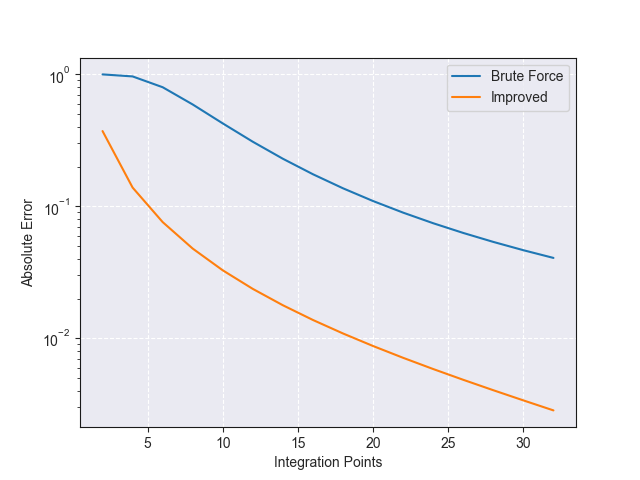
\includegraphics[scale=0.5]{quadrature.png}
    \caption{Figure 1 showing the absolute error comparison between Brute Force Gaussian Quadrature and Improved Gaussian Quadrature for given integration points N.}
    \label{fig:fig1}
\end{figure}
Tabulated results are also included to illustrate the time demands of these methods and the steps required to converge to the correct solution.

\begin{table}[H]
\caption{Brute Force Gaussian Quadrature results for selected values of N integration points. The analytical value of the integral to 8 significant figures is 0.19276571.}
\label{tab:table1}
\begin{ruledtabular}
\begin{tabular}{cccc}
Int Points & Integral Value & Absolute Error & Runtime (s)\\
\hline
 5 & 0.34613906 & 0.79564642 & 0.0006730\\
 10 & 0.11083694 & 0.42501733 & 0.0293350\\
 15 & 0.20963127 & 0.087492507 & 0.3302690 \\
 20 & 0.17162642 & 0.10966315 & 1.7916670 \\
 25 & 0.19037988 & 0.012376866 & 6.8354100\\
 30 & 0.18380124 & 0.046504468 & 20.476816\\
 35 & 0.18946931 & 0.017100542 & 51.388580\\
 \vdots & \vdots & \vdots & \vdots\\
 60 & 0.190527 & 0.011616 & 1360.78\\
\end{tabular}
\end{ruledtabular}
\end{table}

For Brute force Quadrature with up to 60 integration points, we still did not achieve precision to three leading decimal places, illustrating the inneficiencies of this method. By switching to spherical coordinates and using Laguerre-Quadrature for the radial dependency we were able to obtain better results shown in Table 2. We approach the analytical solution with fewer integration points but at the expense of speed.

\begin{table}[H]
\caption{Improved Gaussian Quadrature results for selected values of N integration points. The analytical value of the integral to 8 significant figures is 0.19276571.}
\label{tab:table2}
\begin{ruledtabular}
\begin{tabular}{cccc}
Int Points & Integral Value & Absolute Error & Runtime (s)\\
\hline
 5 & 0.17344965 & 0.10020488 & 0.0019270\\
 10 & 0.18645734 & 0.032725561 & 0.0945780\\
 15 & 0.18975898 & 0.015597842 & 1.0635580\\
 20 & 0.19108178 & 0.0087356352 & 5.9160350\\
 25 & 0.19174074 & 0.0053171840 & 22.829351\\
 30 & 0.19211371 & 0.0033823409 & 67.605018\\
 35 & 0.19234330 & 0.0021913142 & 169.90126\\
\end{tabular}
\end{ruledtabular}
\end{table}

 We then implement Monte-Carlo integration over Cartesian integration boundaries using the uniform distribution to generate our random points and subsequently over spherical boundaries using importance sampling.
\begin{figure}[H]
    \centering
    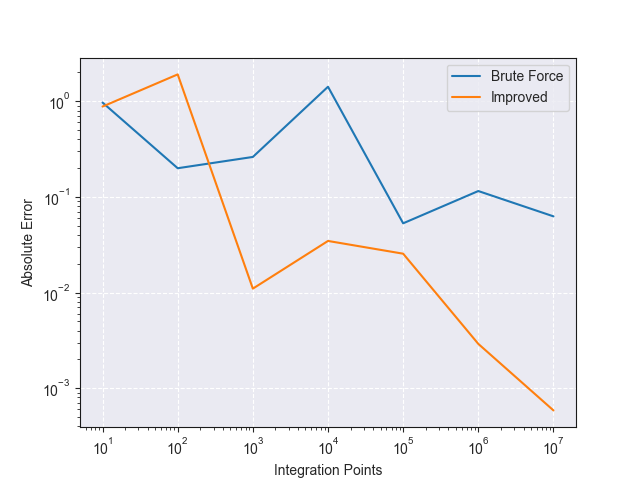
\includegraphics [scale=0.5]{monteerror.png}
    \caption{Figure 2 showing the absolute error of the two Monte Carlo methods for various integration points N}
    \label{fig:fig2}
\end{figure}

\begin{figure}[H]
    \centering
    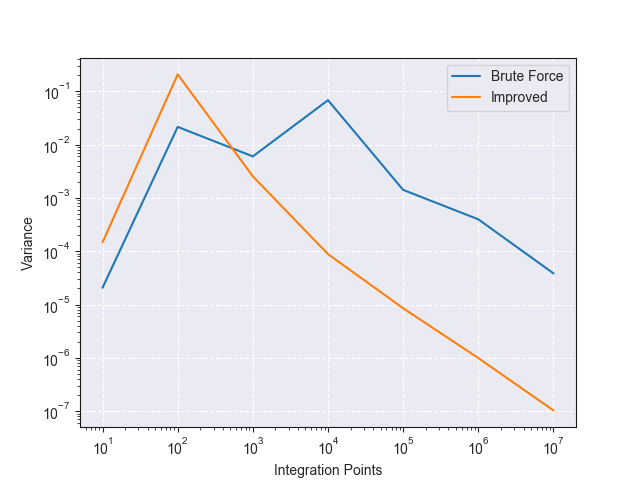
\includegraphics[scale=0.5]{montevariance.png}
    \caption{Figure 3 showing the variance of the two Monte Carlo methods for various integration points N}
    \label{fig:fig3}
\end{figure}
The Monte Carlo results are further displayed in Tables 3 and 4 where runtime can be observed as well.
\begin{table}[H]
\caption{Brute Force Monte Carlo integration results for selected values of N integration points. Integration points are randomly selected from the uniform distribution over interval $[-2.32,2.32]$}
\label{tab:table2}
\begin{ruledtabular}
\begin{tabular}{p{1.3cm} p{1.5cm} p{1.5cm}p{1.5cm} p{1.5cm} }
Int Points & Integral Value & Absolute Error & Variance & Runtime (s)\\
\hline
 $1\times10^{1}$ & 0.00578 & 0.97004 & 0.00002 & 0.00011\\
 $1\times10^{2}$ & 0.15431 & 0.19950 & 0.02149 & 0.00006\\
 $1\times10^{3}$ & 0.14230 & 0.26178 & 0.00600 & 0.00051\\
 $1\times10^{4}$ & 0.46626 & 1.41880 & 0.06798 & 0.00476\\
 $1\times10^{5}$ & 0.20297 & 0.05296 & 0.00141 & 0.03913\\
 $1\times10^{6}$ & 0.21498 & 0.11522 & 0.00040 & 0.39725\\
 $1\times10^{7}$ & 0.20484 & 0.06262 & 0.00004 & 3.97206\\
\end{tabular}
\end{ruledtabular}
\end{table}

\begin{table}[H]
\caption{Improved Monte Carlo integration results using importance sampling. Integration points for $\theta$ and $\phi$ are selected from the uniform distribution over $[0,\pi]$ and $[0,2\pi]$. Integration points for $u$ are selected from the exponential distribution over $[0,\infty)$}
\label{tab:table2}
\begin{ruledtabular}
\begin{tabular}{p{1.3cm} p{1.5cm} p{1.5cm}p{1.5cm} p{1.5cm} }
Int Points & Integral Value & Absolute Error & Variance & Runtime (s)\\
\hline
 $1\times10^{1}$ & 0.02302 & 0.88057 & 0.00015   & 0.00001\\
 $1\times10^{2}$ & 0.56101 & 1.91033 & 0.20719   & 0.00007\\
 $1\times10^{3}$ & 0.19065 & 0.01099 & 0.00254   & 0.00063\\
 $1\times10^{4}$ & 0.18609 & 0.03464 & 0.0000882 & 0.00540\\
 $1\times10^{5}$ & 0.18785 & 0.02548 & 0.0000085 & 0.04815\\
 $1\times10^{6}$ & 0.19221 & 0.00291 & 0.0000010 & 0.50384\\
 $1\times10^{7}$ & 0.19288 & 0.00059 & 0.0000001 & 4.82668\\
\end{tabular}
\end{ruledtabular}
\end{table}

The Monte Carlo solving methods are then solved using parallel cores to observe changes in run time. Finding the optimal number of threads, we then test runtime using various compiler flags, in addition to using this number of threads.
\begin{figure}[H]
    \centering
    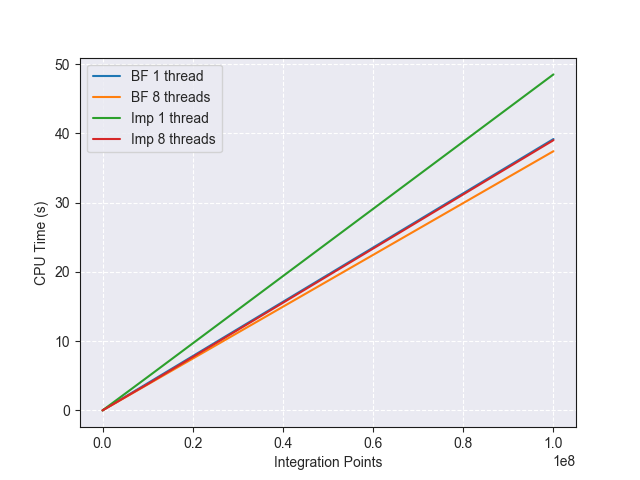
\includegraphics[scale=0.5]{Parallel.png}
    \caption{Figure 4 showing runtime comparison for the Monte Carlo methods when run in parallel. This was done for both methods using 1 and 8 cores.}
    \label{fig:fig4}
\end{figure}

\begin{figure}[H]
    \centering
    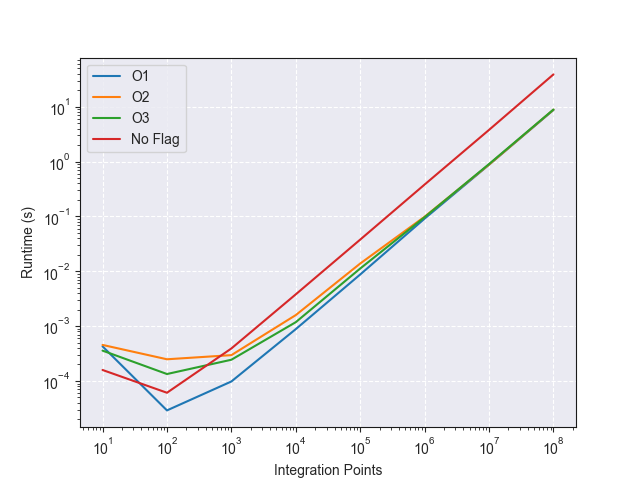
\includegraphics[scale=0.5]{flags.png}
    \caption{Figure 5 showing the runtime comparison for the improved Monte Carlo method. 8 threads were used when running these calculations}
    \label{fig:fig5}
\end{figure}

\section{Discussion}
\label{sec:discussion}
Beginning with Gaussian Quadrature, we see from Figure 1 that transforming to spherical coordinates and using Laguerre Quadrature for the radial component significantly improved accuracy. As displayed in Tables 1 and 2, this increase in accuracy comes at the cost of speed with the improved method running around 3 times as slowly as the brute force method. When compared to the Monte Carlo methods, Quadrature is notable inefficient in terms of runtime. $N=35$ points took the Improved Quadrature method 51.4s while the Improved Monte Carlo method was able to sample $N = 1\times10^{7}$ integration points in just 4.8s. We see from Figures 2 and 3 that selecting our probability distributions to better fit the shape of the data results in better accuracy and lower variance as integration points are increased. We also see that implementing importance sampling when doing Monte Carlo integration gives better results than only using the uniform distribution. The runtime values seen in Tables 3 and 4 show that while accuracy increases, there is only a small CPU time cost. Further run time improvements can be made for Monte Carlo integration by running the program in parallel and including compiler flags for vectorization. Figure 4 shows that by using 8 threads to compute the integral, the Improved Monte Carlo method saw a speed increase of nearly 10 seconds. By adding compiler flags, we see in Figure 5 that the runtime decreased again, this time by nearly 40 seconds. For a low number of integration points, the -O1 compiler flag is optimal while they all converge to a similar performance when integration points approach $N=1\times10^{6}.$

\section{Conclusions}
\label{sec:conclusions}
This paper has shown that the Gaussian quadrature, even though the error scales downwards for increasing grid points, is too inaccurate for practical use. The improved Gaussian quadrature reduces the error by almost one whole order of magnitude, and converges much much faster (in terms of grid points), and is therefore a notable improvement. It is however slow in terms of run time.

The brute force Monte Carlo is very fast, but similarly inaccurate. The improved Monte Carlo gives the best result, as it is both the fastest and the most accurate. In addition, we found that a significant speed up can be achieved by running the code in parallel, and by adding compiler flags to vectorize the code.

In summary, when considering run time and accuracy, one would prefer the improved Monte Carlo method, followed by improved Gaussian, brute force Monte Carlo and finally the brute force Gaussian quadrature.


\newpage
\begin{thebibliography}{}

\bibitem{Lecture1}[(Hjorth-Jensen, 2017)]{MHJ} Hjorth-Jensen, Morten \, Aug 23 2017, "Computational Physics Lectures:Numerical integration, from Newton-Cotes quadrature to Gaussian quadrature" , \url{http://compphysics.github.io/ComputationalPhysics/doc/pub/integrate/pdf/integrate-print.pdf}

\bibitem{Lecture2}[(Hjorth-Jensen, 2019)]{MHJ} Hjorth-Jensen, Morten \, Oct 4 2019, "Computational Physics Lectures: Introduction to Monte Carlo methods" , \url{http://compphysics.github.io/ComputationalPhysics/doc/pub/mcint/pdf/mcint-print.pdf}

\bibitem{Project}[(Hjorth-Jensen, 2019)]{MHJ} Hjorth-Jensen, Morten \, Oct 2019, "Project 3"
\url{http://compphysics.github.io/ComputationalPhysics/doc/Projects/2019/Project3/pdf/Project3.pdf}

\bibitem{codeex}[(Hjorth-Jensen, 2019)]{MHJ} Hjorth-Jensen, Morten \, Oct 2019, "Code Examples"
\url{https://github.com/CompPhysics/ComputationalPhysics/tree/master/doc/Projects/2019/Project3/CodeExamples}

\end{thebibliography}

\section{Appendix}
All source code, data and figures can be found at the github repository: \url{https://github.com/marbjo/FYS4150/tree/master/Project3}

\end{document}
